% 第7章：奇异值分解（输入与输出的正交坐标；构造、形式、唯一性、几何解释、计算与核验；奇异值与矩阵范数）。

\chapter{奇异值分解}
\label{sec:ls-svd}
\label{chap:singular-value-decomposition}

第~\ref{chap:eigen-spectral-decomposition}章的分解都让输入与输出使用同一组基。在这一要求下用标准正交基换基，只有对称矩阵能化为实对角形，正规矩阵能化为分块对角形，一般方阵只能化为分块上三角的实Schur形。矩形矩阵$\bm A\in\mathbb R^{m\times d}$的输入在$\mathbb R^d$中、输出在$\mathbb R^m$中，“同一组基”与特征向量都无从谈起。

本章放宽这一要求，在输入端和输出端各取一组标准正交基。要回答的问题是：这样是否对任意矩阵都能得到对角形？对角元和两组基中哪些由矩阵唯一确定？从这种表示能直接读出矩阵的哪些大小？

第~\ref{sec:svd-orthogonal-coordinates}节先说明为什么要求两组基都标准正交，并写出目标形式。第~\ref{sec:ls-svd-construction}节用对称矩阵$\bm A^\top\bm A$的谱分解构造这两组基，整理分解的几种写法，确定其中的唯一部分与可变部分，用单位球的像解释分解，并给出计算与核验的步骤。第~\ref{sec:ls-svd-matrix-size}节在奇异坐标中比较输出长度，读出谱范数、Frobenius范数、秩与最弱的放大倍数。

本章只依赖第~\ref{chap:eigen-spectral-decomposition}章的谱定理与定号性判据，以及第~\ref{chap:inner-product-spaces}章的标准正交基与第~\ref{chap:normed-inner-product-spaces}章的矩阵范数。由奇异向量选出最佳低秩近似、以及Rayleigh商的极值性质，在第~\ref{chap:matrix-approximation}章讨论；第~\ref{chap:polar-decomposition}章用本章的分解处理奇异矩阵和矩形矩阵的极分解。

\section{输入与输出的正交坐标}
\label{sec:svd-orthogonal-coordinates}

先回忆换基怎样改变一个线性映射的矩阵。设$\bm A\in\mathbb R^{m\times d}$表示映射$\bm x\mapsto\bm A\bm x$。按第~\ref{sec:ls-map-representation}节的约定，若在输入空间$\mathbb R^d$中取新基并排成可逆矩阵$\bm V$，在输出空间$\mathbb R^m$中取新基并排成可逆矩阵$\bm U$，则新坐标下的矩阵为$\bm U^{-1}\bm A\bm V$：先由$\bm V$把输入的新坐标换成标准坐标，作用$\bm A$，再由$\bm U^{-1}$读出输出的新坐标。方阵的相似变换$\bm P^{-1}\bm A\bm P$是$\bm U=\bm V=\bm P$的特殊情形。

两端可以独立换基，自由度就大得多。若$\bm U$、$\bm V$只要求可逆，任何矩阵都能化成只含$0$与$1$的形式。设$r=\operatorname{rank}\bm A$，取$\ker\bm A$的一组基$\bm v_{r+1},\ldots,\bm v_d$，扩充成$\mathbb R^d$的基$\bm v_1,\ldots,\bm v_d$。

这时$\bm A\bm v_1,\ldots,\bm A\bm v_r$线性无关。若$\sum_{i\leq r}c_i\bm A\bm v_i=\bm0$，则
\[
 \sum_{i\leq r}c_i\bm v_i\in\ker\bm A ,
\]
它又是$\bm v_{r+1},\ldots,\bm v_d$的组合，由全体$\bm v_i$线性无关得各$c_i=0$。

把这$r$个向量扩充成$\mathbb R^m$的基并排成$\bm U$，就有
\[
 \bm U^{-1}\bm A\bm V=\begin{bmatrix}\bm I_r&\bm0\\\bm0&\bm0\end{bmatrix}.
\]
这个形式只记录了秩。所有长度信息都被可逆换基吸收掉了，因为一般的可逆矩阵不保持长度。

因此我们要求两组基都标准正交，即$\bm U\in\mathbb R^{m\times m}$与$\bm V\in\mathbb R^{d\times d}$都是正交矩阵。这时$\bm U^{-1}=\bm U^\top$，读坐标只需取内积，而且两端的换基都不改变长度和夹角，变换后的对角元才能表示真正的伸缩倍数。

目标形式是
\[
 \bm U^\top\bm A\bm V=\bm\Sigma ,
\]
其中$\bm\Sigma\in\mathbb R^{m\times d}$只在$(i,i)$位置上可能非零。逐列写出，就是在输入端找标准正交方向$\bm v_i$，在输出端找标准正交方向$\bm u_i$，使
\[
 \bm A\bm v_i=\sigma_i\bm u_i,\qquad\sigma_i\geq0,
\]
其中$i$取$1,\ldots,\min(m,d)$。也就是说，$\bm A$把第$i$个输入方向伸缩$\sigma_i$倍后送到第$i$个输出方向；若输入维数更大，多出的输入基向量还须映到零。

伸缩倍数可以要求非负。若某个对角元为负，把对应的$\bm u_i$换成$-\bm u_i$，输出端仍是标准正交基，而对角元变号。正交矩阵的行列式为$\pm1$，几何上是旋转，或者旋转再加一次反射，例如$\operatorname{diag}(1,-1)$把平面关于第一坐标轴翻转。所以本章所说的输入、输出“转向”可以包含反射，不一概是纯旋转。

这一要求与特征分解的要求不同。特征分解要求$\bm A\bm v$与$\bm v$在同一条直线上，现在只要求被送到另一组标准正交方向中的对应一个。因此它对矩形矩阵有意义，对第~\ref{chap:eigen-spectral-decomposition}章中不能对角化的$\left[\begin{smallmatrix}0.8&1\\0&0.8\end{smallmatrix}\right]$和特征方向几乎平行的$\left[\begin{smallmatrix}0.8&4\\0&0.5\end{smallmatrix}\right]$也有意义。

对称矩阵则提供了现成的例子：若$\bm S=\bm Q\bm\Lambda\bm Q^\top$，取$\bm v_i=\bm q_i$、$\sigma_i=|\lambda_i|$，并在$\lambda_i\geq0$时取$\bm u_i=\bm q_i$、在$\lambda_i<0$时取$\bm u_i=-\bm q_i$，就满足上面的要求。半正定时两组基相同，有负特征值时输出端的相应方向反号。

\section{奇异值分解的构造}
\label{sec:ls-svd-construction}

先看这样的方向若存在，应当满足什么条件。设$\bm x=\sum_ic_i\bm v_i$，则
\[
 \bm A\bm x=\sum_ic_i\sigma_i\bm u_i .
\]
由$\bm u_i$标准正交，
\[
 \bm x^\top\bm A^\top\bm A\bm x=\lVert\bm A\bm x\rVert_2^2=\sum_i\sigma_i^2c_i^2 .
\]
与二次型展开式~\eqref{eq:matrix-analysis-quadratic-spectral-form}比较可知，$\bm v_i$应是对称矩阵$\bm A^\top\bm A$的特征向量，$\sigma_i^2$是对应的特征值。所以构造从$\bm A^\top\bm A$出发。

令$\bm S=\bm A^\top\bm A$。它对称，而且半正定：$\bm x^\top\bm A^\top\bm A\bm x=\lVert\bm A\bm x\rVert_2^2\geq0$。由谱定理（定理~\ref{thm:ls-real-symmetric-spectral}）与定号性判据（定理~\ref{thm:ls-symmetric-definiteness-eigenvalues}），存在$\mathbb R^d$的标准正交基$\bm v_1,\ldots,\bm v_d$使
\[
 \bm A^\top\bm A\bm v_i=\lambda_i\bm v_i,\qquad\lambda_1\geq\cdots\geq\lambda_d\geq0 .
\]

设前$r$个特征值为正，记$\sigma_i=\sqrt{\lambda_i}>0$（$i\leq r$）。其余的$\bm v_j$满足
\[
 \lVert\bm A\bm v_j\rVert_2^2=\bm v_j^\top\bm A^\top\bm A\bm v_j=0 ,
\]
即$\bm A\bm v_j=\bm0$。

对$i\leq r$定义输出方向$\bm u_i=\bm A\bm v_i/\sigma_i$。它们标准正交：
\[
 \bm u_i^\top\bm u_j
 =\frac{\bm v_i^\top\bm A^\top\bm A\bm v_j}{\sigma_i\sigma_j}
 =\frac{\sigma_j^2\,\bm v_i^\top\bm v_j}{\sigma_i\sigma_j}=\delta_{i,j}.
\]
再把$\bm u_1,\dots,\bm u_r$扩充为$\mathbb R^m$的标准正交基$\bm u_1,\ldots,\bm u_m$。这一步处理的是零奇异值：输出端多出的方向不是任何输入的像，只需与已有方向正交。

有了两组方向，就可以写出$\bm A$的作用。把任意$\bm x$展开为$\bm x=\sum_i(\bm v_i^\top\bm x)\bm v_i$，再利用$\bm A\bm v_i=\sigma_i\bm u_i$（$i\leq r$）与$\bm A\bm v_j=\bm0$（$j>r$），得
\[
 \bm A\bm x=\sum_{i=1}^r\sigma_i\bm u_i(\bm v_i^\top\bm x).
\]
这对所有$\bm x$成立，所以$\bm A$是$r$个秩一矩阵之和：
\begin{equation}
 \bm A=\sum_{i=1}^r\sigma_i\bm u_i\bm v_i^\top.
 \label{eq:matrix-analysis-svd-rank-one-sum}
\end{equation}

由这个和式可以读出两个子空间。$\operatorname{range}(\bm A)$由$\bm u_1,\ldots,\bm u_r$张成。又因为$\bm u_i$线性无关且$\sigma_i>0$，$\bm A\bm x=\bm0$当且仅当$\bm v_i^\top\bm x=0$（$i\leq r$），所以$\ker\bm A$由$\bm v_{r+1},\ldots,\bm v_d$张成。于是$r=\operatorname{rank}\bm A$。

把这些向量排成矩阵，就得到下面的结论。

\begin{theorem}[SVD的存在]
\label{thm:ls-svd-existence}
对任意$\bm A\in\mathbb R^{m\times d}$，存在正交矩阵$\bm U\in\mathbb R^{m\times m}$、$\bm V\in\mathbb R^{d\times d}$与对角矩阵$\bm\Sigma\in\mathbb R^{m\times d}$，使$\bm A=\bm U\bm\Sigma\bm V^\top$；$\bm\Sigma$的对角元$\sigma_1\geq\cdots\geq\sigma_{\min(m,d)}\geq0$，其中恰有$\operatorname{rank}\bm A$个为正。
\end{theorem}

定理中的$\bm\Sigma$与$\bm A$形状相同，“对角”指只有$(i,i)$位置的元素可能非零。这种分解有专门的名称。

\begin{definition}[奇异值分解]
\label{def:matrix-analysis-svd}
称
\begin{equation}
 \bm A=\bm U\bm\Sigma\bm V^\top
 \label{eq:matrix-analysis-svd}
\end{equation}
为$\bm A$的\term{奇异值分解}（singular value decomposition, SVD），$\bm\Sigma$的对角元$\sigma_i$称为\term{奇异值}（singular value），$\bm U$、$\bm V$的列$\bm u_i$、$\bm v_i$分别称为左、右\term{奇异向量}（singular vector）。
\end{definition}

图~\ref{fig:ls-svd-construction}把构造拆成三步：形成$\bm A^\top\bm A$；由谱定理将其对角化；开方得到奇异值，再由$\bm u_i=\bm A\bm v_i/\sigma_i$得到左奇异向量。

\begin{figure*}[htbp]
  \centering
  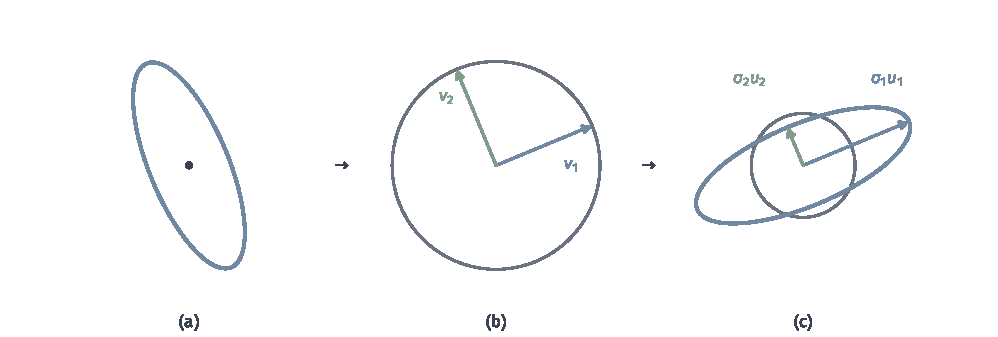
\includegraphics[width=168.998mm]{figures/00-shared/mathematical-preliminaries-upper/02-linear-spaces/matplotlib/ls-svd-construction/ls-svd-construction.pdf}
  \caption{SVD的三步构造。取$\bm A=\left[\begin{smallmatrix}2&0.5\\0.5&1\end{smallmatrix}\right]$，$\bm G=\bm A^\top\bm A=\left[\begin{smallmatrix}4.25&1.5\\1.5&1.25\end{smallmatrix}\right]$。(a)~二次型等值线$\bm x^\top\bm G\bm x=2$；(b)~$\bm G$的标准正交特征方向$\bm v_1,\bm v_2$，特征值约为$4.87,0.63$；(c)~单位圆及其在$\bm A$下的像，箭头为$\bm A\bm v_i=\sigma_i\bm u_i$，$\sigma_i=\sqrt{\lambda_i}\approx2.21,0.79$。各面板单独设定显示尺度。}
  \label{fig:ls-svd-construction}
\end{figure*}

左奇异向量与输出端也有对称的关系。对$i\leq r$，
\[
 \bm A^\top\bm u_i=\bm A^\top\bm A\bm v_i/\sigma_i=\sigma_i\bm v_i .
\]
对$i>r$，$\bm u_i$与$\operatorname{range}(\bm A)$正交，故对任意$\bm x$有
\[
 (\bm A^\top\bm u_i)^\top\bm x=\bm u_i^\top\bm A\bm x=0 ,
\]
即$\bm A^\top\bm u_i=\bm0$。于是
\begin{equation}
 \bm A^\top\bm u_i=\sigma_i\bm v_i,\qquad
 \bm A\bm A^\top\bm u_i=\sigma_i^2\bm u_i\qquad(i\leq r),
 \label{eq:ls-svd-transpose-relation}
\end{equation}
而$i>r$时$\bm A\bm A^\top\bm u_i=\bm0$。

也就是说，$\bm u_1,\ldots,\bm u_m$是$\bm A\bm A^\top$的一组标准正交特征向量，特征值依次为$\sigma_1^2,\ldots,\sigma_r^2$与$m-r$个零。$\bm A^\top\bm A$与$\bm A\bm A^\top$因而有相同的正特征值，分别在输入端与输出端给出奇异方向。

构造路线只用于证明存在性，并不意味着数值计算应当显式形成$\bm A^\top\bm A$；这一点在第~\ref{sec:svd-computation}节说明。

\subsection{奇异值分解的形式}
\label{sec:svd-forms}

定理~\ref{thm:ls-svd-existence}中的$\bm U$、$\bm V$都是方阵，这是\emph{完整}分解，它同时给出两端的全部正交方向：$\bm v_{r+1},\ldots,\bm v_d$张成$\ker\bm A$，$\bm u_{r+1},\ldots,\bm u_m$张成$\operatorname{range}(\bm A)$的正交补。三个因子的形状依次为$m\times m$、$m\times d$与$d\times d$。

许多计算只用到前$p=\min(m,d)$列。令$\bm U_p=[\bm u_1,\ldots,\bm u_p]\in\mathbb R^{m\times p}$、$\bm V_p=[\bm v_1,\ldots,\bm v_p]\in\mathbb R^{d\times p}$、$\bm\Sigma_p=\operatorname{diag}(\sigma_1,\ldots,\sigma_p)\in\mathbb R^{p\times p}$，则
\[
 \bm A=\bm U_p\bm\Sigma_p\bm V_p^\top ,
\]
称为\term{薄奇异值分解}（thin SVD），也称经济型分解。它由完整分解删去$\bm\Sigma$中全为零的那些行或列，连同与之相乘的$\bm U$或$\bm V$的列得到，乘积不变。$m\geq d$时删去的是$\bm U$的后$m-d$列，$m<d$时删去的是$\bm V$的后$d-m$列。

若只保留正奇异值，令$\bm U_r$、$\bm V_r$分别由前$r$个左、右奇异向量组成，$\bm\Sigma_r=\operatorname{diag}(\sigma_1,\ldots,\sigma_r)$，则
\[
 \begin{gathered}
 \bm A=\bm U_r\bm\Sigma_r\bm V_r^\top,\\
 \bm U_r\in\mathbb R^{m\times r},\quad\bm\Sigma_r\in\mathbb R^{r\times r},\quad\bm V_r\in\mathbb R^{d\times r},
 \end{gathered}
\]
这就是和式~\eqref{eq:matrix-analysis-svd-rank-one-sum}的矩阵写法，称为秩分解形式。

三种写法给出同一个矩阵，区别在于是否保留零伸缩的方向。秩分解只描述$\bm A$真正起作用的$r$对方向，$\bm U_r$与$\bm V_r$只是列标准正交，不再是方阵；零空间与输出端正交补的基要从完整分解中读取。薄分解在$r<p$时仍保留奇异值为零的列。三者都是$\bm A$的精确表示；只保留前$k<r$项、从而改变矩阵的截断近似，在第~\ref{chap:matrix-approximation}章讨论。

\subsection{奇异值分解的唯一性}
\label{sec:svd-uniqueness}

构造中有两处选择：$\bm A^\top\bm A$的标准正交特征基怎样选，以及输出端怎样补全。所以奇异值分解一般不唯一。本小节确定哪些部分由$\bm A$唯一决定。

先看奇异值。设$\bm A=\bm U\bm\Sigma\bm V^\top$是任意一个满足定理~\ref{thm:ls-svd-existence}的分解，则
\[
 \bm A^\top\bm A=\bm V(\bm\Sigma^\top\bm\Sigma)\bm V^\top ,
\]
其中$\bm\Sigma^\top\bm\Sigma$是$d$阶对角矩阵，对角元为$\sigma_1^2,\ldots,\sigma_{\min(m,d)}^2$，$d>m$时再补$d-m$个零。

$\bm V^\top=\bm V^{-1}$，所以$\bm A^\top\bm A$与$\bm\Sigma^\top\bm\Sigma$相似。由定理~\ref{thm:ls-spectrum-similarity-invariance}，二者有相同的特征多项式，$\sigma_i^2$连同重数恰是$\bm A^\top\bm A$的特征值。

$\bm A^\top\bm A$只依赖$\bm A$，而$\sigma_i$是这些特征值降序排列后的非负平方根，因此与分解的选取无关：正奇异值是$\bm A^\top\bm A$正特征值的平方根，其余为零。

奇异向量则可以变化。最简单的变化是把一对$\bm u_i,\bm v_i$同时变号：乘积$\sigma_i\bm u_i\bm v_i^\top$不变，两组向量仍各自标准正交。

奇异值重复时变化更多，例如$\bm A=\bm I_2$的奇异值都是$1$，对任意正交矩阵$\bm R$，$\bm I_2=\bm R\bm I_2\bm R^\top$都是奇异值分解。但两端不能各自独立地换：$\bm R_1\bm I_2\bm R_2^\top=\bm I_2$迫使$\bm R_1=\bm R_2$。下面的定理说明，这些例子已经包括了全部的自由度。

\begin{theorem}[奇异值分解的唯一性范围]
\label{thm:svd-uniqueness}
设$\bm A\in\mathbb R^{m\times d}$，$r=\operatorname{rank}\bm A$，$\bm A=\bm U\bm\Sigma\bm V^\top$是一个奇异值分解。对每个正奇异值$\sigma$，把$\bm V$、$\bm U$中满足$\sigma_i=\sigma$的列分别排成$\bm V_\sigma$、$\bm U_\sigma$；把$\bm V$的后$d-r$列与$\bm U$的后$m-r$列分别排成$\bm V_0$、$\bm U_0$。则：
\begin{enumerate}
 \item $\bm V_\sigma$与$\bm U_\sigma$的列空间分别是$\ker(\bm A^\top\bm A-\sigma^2\bm I)$与$\ker(\bm A\bm A^\top-\sigma^2\bm I)$，且$\bm U_\sigma=\bm A\bm V_\sigma/\sigma$；$\bm V_0$与$\bm U_0$的列空间分别是$\ker\bm A$与$\operatorname{range}(\bm A)^\perp$。
 \item 若$\bm A=\bm U'\bm\Sigma\bm V'^\top$是另一个奇异值分解，相应的分组记为$\bm V'_\sigma$等，则对每个正奇异值$\sigma$存在正交矩阵$\bm R_\sigma$，使
 \[
  \bm V'_\sigma=\bm V_\sigma\bm R_\sigma,\qquad\bm U'_\sigma=\bm U_\sigma\bm R_\sigma .
 \]
 \item 反过来，把$\bm V_0$、$\bm U_0$分别换成$\ker\bm A$与$\operatorname{range}(\bm A)^\perp$的任意标准正交基，或对某个$\sigma$同时右乘同一个正交矩阵$\bm R_\sigma$，所得仍是奇异值分解。
\end{enumerate}
特别地，每个正奇异值对应的项$\sigma\bm U_\sigma\bm V_\sigma^\top$由$\bm A$唯一确定。
\end{theorem}
\begin{proof}
(1)由$\bm A\bm V=\bm U\bm\Sigma$与$\bm A^\top\bm U=\bm V\bm\Sigma^\top$逐列读出
\[
 \bm A\bm v_i=\sigma_i\bm u_i,\qquad\bm A^\top\bm u_i=\sigma_i\bm v_i\qquad(i\leq\min(m,d)),
\]
其余列被$\bm A$或$\bm A^\top$送到零。于是
\[
 \bm A^\top\bm A\bm v_i=\sigma_i^2\bm v_i ,
\]
$\bm V$的各列是$\bm A^\top\bm A$的一组标准正交特征基，特征值依次为$\sigma_1^2,\ldots$，不足$d$个时补零。由谱投影定理~\ref{thm:ls-spectral-projections}的第一条，特征空间$\ker(\bm A^\top\bm A-\sigma^2\bm I)$恰由满足$\sigma_i^2=\sigma^2$的那些列张成，即$\bm V_\sigma$的列空间。

对$\bm A\bm A^\top=\bm U(\bm\Sigma\bm\Sigma^\top)\bm U^\top$同样讨论，得$\bm U_\sigma$的列空间。由$\bm A\bm v_i=\sigma\bm u_i$得$\bm U_\sigma=\bm A\bm V_\sigma/\sigma$。

$\bm V_0$的$d-r$列都满足$\bm A\bm v_i=\bm0$，彼此标准正交，而$\dim\ker\bm A=d-r$，所以它们是$\ker\bm A$的基。$\bm U_0$的$m-r$列与$\bm u_1,\ldots,\bm u_r$正交，后者张成$\operatorname{range}(\bm A)$，而$\dim\operatorname{range}(\bm A)^\perp=m-r$，所以它们是$\operatorname{range}(\bm A)^\perp$的基。

(2)由第一条，$\bm V_\sigma$与$\bm V'_\sigma$的列是同一个子空间的两组标准正交基。与谱投影定理第四条的证明相同，$\bm R_\sigma=\bm V_\sigma^\top\bm V'_\sigma$是正交矩阵，且$\bm V'_\sigma=\bm V_\sigma\bm R_\sigma$。再由第一条用于两个分解，
\[
 \bm U'_\sigma=\frac1\sigma\bm A\bm V'_\sigma=\frac1\sigma\bm A\bm V_\sigma\bm R_\sigma=\bm U_\sigma\bm R_\sigma .
\]

(3)分解按奇异值分组可以写成
\[
 \bm A=\sum_{\sigma>0}\sigma\bm U_\sigma\bm V_\sigma^\top ,
\]
其中不出现$\bm V_0$与$\bm U_0$，所以替换它们不改变乘积。新的列仍与其余列正交：$\ker\bm A$是$\operatorname{span}\{\bm v_1,\ldots,\bm v_r\}$的正交补，$\operatorname{range}(\bm A)^\perp$是$\operatorname{span}\{\bm u_1,\ldots,\bm u_r\}$的正交补，所以$\bm U$、$\bm V$仍是正交矩阵。

同时右乘$\bm R_\sigma$时，
\[
 \bm U_\sigma\bm R_\sigma(\bm V_\sigma\bm R_\sigma)^\top=\bm U_\sigma\bm V_\sigma^\top ,
\]
乘积不变，列仍标准正交。

最后一句由第二条得到：
\[
 \bm U'_\sigma\bm V_\sigma'^\top=\bm U_\sigma\bm R_\sigma\bm R_\sigma^\top\bm V_\sigma^\top=\bm U_\sigma\bm V_\sigma^\top .
\]
\end{proof}

于是，奇异值和每个正奇异值对应的左、右奇异子空间都由$\bm A$决定；同一个奇异值内部，左右两组基必须用同一个正交矩阵一起旋转，因为它们由$\bm u=\bm A\bm v/\sigma$配对。零奇异值的两部分则彼此独立，可以分别任意选取。若正奇异值互不相同，每个$\bm R_\sigma$都是$1\times1$的正交矩阵$\pm1$，奇异向量对只差一个公共的符号。这与第~\ref{sec:ls-spectral-projections}节的情形相仿：具体的向量可以变，子空间和合并后的项不变。

\subsection{奇异值分解的几何解释}
\label{sec:svd-geometry}


几何上，SVD把$\bm A$的作用拆成三步：$\bm V^\top$把输入写成右奇异方向上的坐标，$\bm\Sigma$把第$i$个坐标乘以$\sigma_i$，$\bm U$再把结果放到输出空间的左奇异方向上。正交矩阵保持长度，所以只有中间一步改变长度。于是$\bm A$把输入端的单位球映成输出空间中一个椭球；秩亏时这个椭球落在低维子空间内。

具体地，单位球中的$\bm x=\sum_ic_i\bm v_i$满足$\sum_ic_i^2\leq1$，其像为
\[
 \bm y=\sum_{i\leq r}\sigma_ic_i\bm u_i ,
\]
它落在$\operatorname{span}\{\bm u_1,\ldots,\bm u_r\}$中。坐标$y_i=\bm u_i^\top\bm y=\sigma_ic_i$满足
\[
 \sum_{i\leq r}(y_i/\sigma_i)^2=\sum_{i\leq r}c_i^2\leq1 .
\]

反过来，该子空间中满足这一不等式的$\bm y$是$\bm x=\sum_{i\leq r}(y_i/\sigma_i)\bm v_i$的像，而这个$\bm x$在单位球中。所以像恰为
\[
 \Bigl\{\bm y\in\operatorname{span}\{\bm u_1,\ldots,\bm u_r\}:\ \sum_{i=1}^r\frac{(\bm u_i^\top\bm y)^2}{\sigma_i^2}\leq1\Bigr\},
\]
即以$\sigma_i\bm u_i$为半轴的椭球：$\bm v_i$方向的单位向量被送到半轴端点$\sigma_i\bm u_i$。

若$r<d$，单位球面上的点也可能映到这个椭球的内部，例如$(\bm v_1+\bm v_d)/\sqrt2$被送到$\sigma_1\bm u_1/\sqrt2$，所以这里用单位球而不是球面描述整个像。

按这一图像，最长半轴就是最强的放大，第~\ref{sec:ls-svd-matrix-size}节将证明它等于$\lVert\bm A\rVert_2$，各半轴长度的平方和等于$\lVert\bm A\rVert_{\mathrm F}^2$。图~\ref{fig:matrix-analysis-svd-geometry}用二维旋转矩阵$\bm R(\theta)=\left[\begin{smallmatrix}\cos\theta&-\sin\theta\\\sin\theta&\cos\theta\end{smallmatrix}\right]$构造了一个输入方向与输出方向不同的例子。

\begin{figure*}[htbp]
  \centering
  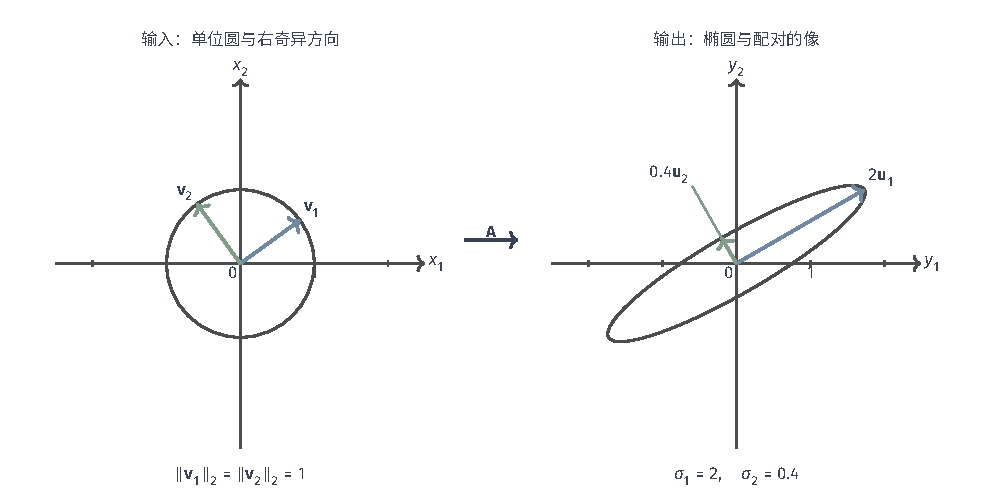
\includegraphics[width=168.998mm]{figures/00-shared/mathematical-preliminaries-upper/02-linear-spaces/tikz/matrix-analysis-svd-geometry/figure.pdf}
  \caption{矩阵$\bm A=\bm R(\pi/6)\operatorname{diag}(2,0.4)\bm R(\pi/5)^\top$
  将单位圆变为椭圆。蓝、绿分别对应两个奇异方向；同色箭头在左侧标出$\bm v_i$，
  在右侧标出其像$\sigma_i\bm u_i$。两侧坐标比例相同。奇异值决定长度变化，左右方向可以不同，
  因而这不是沿特征方向的同空间缩放。图为教学构造。}
  \label{fig:matrix-analysis-svd-geometry}
\end{figure*}

\subsection{奇异值分解的计算与核验}
\label{sec:svd-computation}
\phantomsection
\label{sec:svd-verification-geometry}

存在性定理的证明已经给出一条构造路线。对手算规模的矩阵$\bm A\in\mathbb R^{m\times d}$，可以按以下次序求出三个因子。先求对称半正定矩阵$\bm A^\top\bm A$的全部特征值，按降序记为$\lambda_1\geq\cdots\geq\lambda_d\geq0$，开方得到奇异值$\sigma_i=\sqrt{\lambda_i}$，正奇异值的个数就是$r=\operatorname{rank}\bm A$。再按第~\ref{sec:ls-spectral-decomposition-computation}节的方法求$\bm A^\top\bm A$的一组标准正交特征向量$\bm v_1,\ldots,\bm v_d$，排成$\bm V$，次序与特征值一致。然后对$i\leq r$令$\bm u_i=\bm A\bm v_i/\sigma_i$。最后若$r<m$，把$\bm u_1,\ldots,\bm u_r$补成$\mathbb R^m$的标准正交基，例如取$\ker\bm A^\top$的一组标准正交基作为$\bm u_{r+1},\ldots,\bm u_m$，排成$\bm U$。

第三步得到的向量自动标准正交，不必再正交化。对$i,j\leq r$，
\[
 \bm u_i^\top\bm u_j=\frac{\bm v_i^\top\bm A^\top\bm A\bm v_j}{\sigma_i\sigma_j}=\frac{\lambda_j\,\bm v_i^\top\bm v_j}{\sigma_i\sigma_j},
\]
$i\neq j$时为零，$i=j$时为$\lambda_i/\sigma_i^2=1$。补全的方向取在$\ker\bm A^\top=\operatorname{range}(\bm A)^\perp$中，与前$r$个方向自动垂直。

算出三个因子之后，或者拿到别人给出的一组因子时，要逐项核验。需要检查三件事：$\bm U^\top\bm U=\bm I$与$\bm V^\top\bm V=\bm I$；$\bm\Sigma$只有非负的对角元，并按降序排列；$\bm A\bm V=\bm U\bm\Sigma$，逐列看就是$\bm A\bm v_i=\sigma_i\bm u_i$。三项都成立时，在$\bm A\bm V=\bm U\bm\Sigma$两边右乘$\bm V^\top$，由$\bm V\bm V^\top=\bm I$即得$\bm A=\bm U\bm\Sigma\bm V^\top$。

正交性不能省略。若只核对乘积，任何分解$\bm A=\bm B\bm C$都可以写成$\bm U=\bm B$、$\bm\Sigma=\bm I$、$\bm V^\top=\bm C$的形式，却与奇异值毫无关系。另一方面，$\bm A^\top\bm U=\bm V\bm\Sigma^\top$由前三项推出，可以作为附加检查，它同时检验左奇异向量是否是$\bm A\bm A^\top$的特征向量。

\begin{example}[二阶矩阵的奇异值分解与核验]
\label{ex:svd-two-by-two-check}
下面用以下不对称的二阶矩阵演示：
\[
 \bm A=\begin{bmatrix}3&0\\4&5\end{bmatrix}.
\]
我们按上面的次序求出它的奇异值分解，再按三项逐一核验。

构造从对称矩阵$\bm A^\top\bm A$出发：
\[
 \bm A^\top\bm A=\begin{bmatrix}25&20\\20&25\end{bmatrix}.
\]
它的特征多项式为
\[
 (z-25)^2-400=(z-45)(z-5),
\]
特征值为$45$与$5$，对应的单位特征向量为$\bm v_1=(1,1)^\top/\sqrt2$与$\bm v_2=(1,-1)^\top/\sqrt2$。它们就是右奇异向量。特征值开方得到奇异值
\[
 \sigma_1=\sqrt{45}=3\sqrt5,\qquad\sigma_2=\sqrt5 .
\]

输出端的方向不必另解方程，由$\bm u_i=\bm A\bm v_i/\sigma_i$直接得到：
\[
 \begin{aligned}
 \bm u_1&=\frac{1}{3\sqrt5}\cdot\frac1{\sqrt2}\begin{bmatrix}3\\9\end{bmatrix}=\frac1{\sqrt{10}}\begin{bmatrix}1\\3\end{bmatrix},\\
 \bm u_2&=\frac{1}{\sqrt5}\cdot\frac1{\sqrt2}\begin{bmatrix}3\\-1\end{bmatrix}=\frac1{\sqrt{10}}\begin{bmatrix}3\\-1\end{bmatrix}.
 \end{aligned}
\]

接着逐项核验。正交性：
\[
 \bm u_1^\top\bm u_2=(3-3)/10=0 ,
\]
两者长度为$1$，$\bm v_1,\bm v_2$同样标准正交。对角元：$\sigma_1\geq\sigma_2>0$，非负且降序。

乘积：按秩一和式重建，
\[
 \begin{aligned}
 \sigma_1\bm u_1\bm v_1^\top+\sigma_2\bm u_2\bm v_2^\top
 &=\frac32\begin{bmatrix}1&1\\3&3\end{bmatrix}+\frac12\begin{bmatrix}3&-3\\-1&1\end{bmatrix}\\
 &=\begin{bmatrix}3&0\\4&5\end{bmatrix}=\bm A ,
 \end{aligned}
\]
其中$\sigma_1/\sqrt{20}=3/2$，$\sigma_2/\sqrt{20}=1/2$。

作为附加检查，
\[
 \bm A^\top\bm u_1=(15,15)^\top/\sqrt{10}=3\sqrt5\,\bm v_1 ,
\]
与式~\eqref{eq:ls-svd-transpose-relation}相符。

有了分解，第~\ref{sec:ls-svd-matrix-size}节将说明的几项大小就能直接读出：$\lVert\bm A\rVert_2=3\sqrt5\approx6.71$；$\lVert\bm A\rVert_{\mathrm F}^2=45+5=50$，与逐元素平方和$9+16+25$一致；两个奇异值都为正，$\bm A$可逆，且$\lVert\bm A^{-1}\rVert_2=1/\sqrt5$。
\end{example}

这个矩阵不对称，它的特征值是对角元$3$与$5$，与奇异值$6.71$、$2.24$都不同。特征值描述沿特征方向的倍数，奇异值描述把输入方向送到另一组正交方向时的倍数。对称半正定矩阵的奇异值就是它的特征值（第~\ref{sec:svd-orthogonal-coordinates}节），一般矩阵二者不同。

\paragraph{数值计算中的核验}

上面的构造与核验都是精确的代数运算。数值软件返回的因子$\widehat{\bm U}$、$\widehat{\bm\Sigma}$、$\widehat{\bm V}$带有舍入误差，各项等式只能近似成立，所以要分别报告两类残差。一类是重建误差
\[
 \lVert\bm A-\widehat{\bm U}\widehat{\bm\Sigma}\widehat{\bm V}^\top\rVert/\lVert\bm A\rVert ,
\]
另一类是正交性误差
\[
 \lVert\widehat{\bm U}^\top\widehat{\bm U}-\bm I\rVert,\qquad\lVert\widehat{\bm V}^\top\widehat{\bm V}-\bm I\rVert .
\]

两类残差不能互相代替。前面的例子已经说明，重建误差为零并不保证因子正交；反过来，两组列都正交、乘积却不等于$\bm A$，也只说明找到了某种正交矩阵。只有两类残差都小，才能把$\widehat{\bm\Sigma}$的对角元当作$\bm A$的奇异值的近似值；它们离真实奇异值有多远，由第~\ref{chap:condition-and-spectral-perturbation}章的奇异值扰动界判断。

构造路线从$\bm A^\top\bm A$出发，这条路线适合证明存在性，却不宜照搬到数值计算中。$\bm A^\top\bm A$的特征值是$\sigma_i^2$，最大与最小奇异值之比在其中变成平方，小奇异值相对于大奇异值变得更小，容易被舍入误差淹没。第~\ref{sec:ls-ls-regularization-sensitivity}节以最小二乘的正规方程为例分析这种平方带来的误差风险。实际计算奇异值分解的算法直接作用于$\bm A$本身，其构造与误差分析不在本书展开。

\section{奇异值与矩阵范数}
\label{sec:ls-svd-matrix-size}

第~\ref{sec:ls-frobenius-norm}节与第~\ref{sec:ls-matrix-norms}节分别定义了Frobenius范数与谱范数，但没有给出谱范数的算法。奇异值分解把这个问题化为比较坐标的平方和。

为了统一书写，把零伸缩也计入。对$\bm x\in\mathbb R^d$，写$\bm x=\sum_{i=1}^dc_i\bm v_i$，其中$c_i=\bm v_i^\top\bm x$，并约定$i>\min(m,d)$时$\sigma_i=0$。于是对每个$i\leq d$都有$\bm A\bm v_i=\sigma_i\bm u_i$或$\bm A\bm v_i=\bm0$，后者对应$\sigma_i=0$。由$\bm u_i$标准正交与$\bm v_i$标准正交，
\begin{equation}
 \lVert\bm A\bm x\rVert_2^2=\sum_{i=1}^d\sigma_i^2c_i^2,\qquad
 \lVert\bm x\rVert_2^2=\sum_{i=1}^dc_i^2 .
 \label{eq:svd-output-length}
\end{equation}

输出长度的平方是各$\sigma_i^2$以$c_i^2$为权的和。各$\sigma_i^2$都不超过最大的$\sigma_1^2$，也不小于补零后最小的$\sigma_d^2$，所以
\[
 \sigma_d\lVert\bm x\rVert_2\leq\lVert\bm A\bm x\rVert_2\leq\sigma_1\lVert\bm x\rVert_2 ,
\]
这里$d>m$或$\operatorname{rank}\bm A<d$时$\sigma_d=0$。取$\bm x=\bm v_1$时只有$c_1=1$，上界取等号；取$\bm x=\bm v_d$时下界取等号。这一比较只用到坐标平方和，不涉及任何极值原理。

由上界及其可达性，单位输入的最大输出长度就是$\sigma_1$。

Frobenius范数则由迹的循环性得到：
\[
 \begin{aligned}
 \lVert\bm A\rVert_{\mathrm F}^2&=\operatorname{tr}(\bm A^\top\bm A)=\operatorname{tr}\bigl(\bm V(\bm\Sigma^\top\bm\Sigma)\bm V^\top\bigr)\\
 &=\operatorname{tr}(\bm\Sigma^\top\bm\Sigma\bm V^\top\bm V)=\sum_i\sigma_i^2 .
 \end{aligned}
\]
因此
\begin{align}
 \lVert\bm A\rVert_2&=\sigma_1,
 \label{eq:matrix-analysis-spectral-norm}\\
 \lVert\bm A\rVert_{\mathrm F}&=\Bigl(\sum_{i=1}^r\sigma_i^2\Bigr)^{1/2}.
 \label{eq:matrix-analysis-frobenius-norm}
\end{align}
正奇异值的个数等于$\operatorname{rank}\bm A$，这已在构造中证明。谱范数只看最强的一个伸缩，Frobenius范数把全部伸缩的平方加在一起，所以
\[
 \lVert\bm A\rVert_2\leq\lVert\bm A\rVert_{\mathrm F}\leq\sqrt r\,\lVert\bm A\rVert_2 .
\]

下界在秩亏时为零，并不提供信息。$\ker\bm A$中的非零输入被送到零，它们的输出长度不说明$\bm A$在其他方向上作用多弱。有意义的问题是在$\ker\bm A$的正交补$\operatorname{span}\{\bm v_1,\ldots,\bm v_r\}$上，单位输入至少被送出多远。满列秩时$\ker\bm A=\{\bm0\}$，这个正交补就是整个输入空间。可逆方阵的逆矩阵则把每个伸缩倍数倒过来，最弱的放大变成逆矩阵最强的放大。下面的定理汇总这几项读数。

\begin{theorem}[最小奇异值与逆矩阵的范数]
\label{thm:ls-svd-singular-value-norms}
设$\bm A\in\mathbb R^{m\times d}$的秩为$r\geq1$，奇异值分解如定理~\ref{thm:ls-svd-existence}所示。
\begin{enumerate}
 \item 对$\ker\bm A$的正交补中的任意$\bm x$，$\lVert\bm A\bm x\rVert_2\geq\sigma_r\lVert\bm x\rVert_2$，等号在$\bm x=\bm v_r$时成立。
 \item 若$\bm A$满列秩，即$r=d\leq m$，则对所有$\bm x\in\mathbb R^d$，$\lVert\bm A\bm x\rVert_2\geq\sigma_d\lVert\bm x\rVert_2$，且
 \[
  \min_{\lVert\bm x\rVert_2=1}\lVert\bm A\bm x\rVert_2=\sigma_d>0 .
 \]
 \item 若$\bm A$是可逆方阵（$m=d=r$），则$\bm A^{-1}=\sum_{i=1}^d\sigma_i^{-1}\bm v_i\bm u_i^\top$，并且
 \begin{equation}
  \lVert\bm A^{-1}\rVert_2=\frac1{\sigma_d}.
  \label{eq:ls-svd-inverse-norm}
 \end{equation}
\end{enumerate}
\end{theorem}
\begin{proof}
由构造，$\ker\bm A$由$\bm v_{r+1},\ldots,\bm v_d$张成，其正交补由$\bm v_1,\ldots,\bm v_r$张成。对其中的$\bm x=\sum_{i\leq r}c_i\bm v_i$，由式~\eqref{eq:svd-output-length}，
\[
 \lVert\bm A\bm x\rVert_2^2=\sum_{i\leq r}\sigma_i^2c_i^2\geq\sigma_r^2\sum_{i\leq r}c_i^2=\sigma_r^2\lVert\bm x\rVert_2^2 ,
\]
其中用到$\sigma_i\geq\sigma_r$（$i\leq r$）；取$\bm x=\bm v_r$时只有$c_r=1$，等号成立。这是第一条。

满列秩时正交补就是$\mathbb R^d$，且$\sigma_r=\sigma_d>0$，第一条即给出第二条。

对第三条，令$\bm B=\sum_i\sigma_i^{-1}\bm v_i\bm u_i^\top$。由$\bm v_i^\top\bm v_j=\delta_{i,j}$，
\[
 \begin{aligned}
 \bm A\bm B&=\sum_{i,j}\sigma_i\sigma_j^{-1}\bm u_i(\bm v_i^\top\bm v_j)\bm u_j^\top\\
 &=\sum_i\bm u_i\bm u_i^\top=\bm U\bm U^\top=\bm I,
 \end{aligned}
\]
方阵的右逆就是逆，所以$\bm B=\bm A^{-1}$。

这个和式本身就是$\bm A^{-1}$的奇异值分解：右奇异向量为$\bm u_i$，左奇异向量为$\bm v_i$，奇异值为$\sigma_i^{-1}$，其中最大的是$\sigma_d^{-1}$。由式~\eqref{eq:matrix-analysis-spectral-norm}，$\lVert\bm A^{-1}\rVert_2=1/\sigma_d$。
\end{proof}

满列秩只保证最小放大倍数为正，并不保证它不太小。式~\eqref{eq:ls-svd-inverse-norm}说明，最小奇异值越小，逆矩阵把输出端的误差放大得越厉害。最大奇异值衡量最强的放大，最小奇异值衡量最弱的放大，二者之比就是第~\ref{sec:ls-matrix-condition-number}节的矩阵条件数，它决定线性方程的解对数据误差有多敏感。

当$r<d$时（$m<d$时总是如此），存在非零输入被送到零，单位输入的最小输出长度为零，这时只能在零空间的正交补上谈最弱的放大。最弱放大的方向$\bm v_d$也有直接用处：第~\ref{sec:linear-algebra-homogeneous-estimation}节的齐次最小二乘在单位向量中最小化$\lVert\bm A\bm x\rVert_2$，由上面的下界及其取等条件，最优解就是$\bm v_d$。

本节的上下界是对单个输入的比较。若要在所有$k$维子空间中挑出保留输出能量最多的一个，就需要比较子空间，这是第~\ref{chap:matrix-approximation}章用Rayleigh商和迹极值处理的最优选择问题。

\FloatBarrier
\section{本章小结}
\label{sec:svd-chapter-summary}

本章开头问：输入、输出各取一组标准正交基时，是否任何矩阵都能化为对角形？答案是肯定的。由$\bm A^\top\bm A$的谱分解取右奇异向量$\bm v_i$，开方得到奇异值$\sigma_i$，再令$\bm u_i=\bm A\bm v_i/\sigma_i$并补全，就得到$\bm A=\bm U\bm\Sigma\bm V^\top$，即$\bm A\bm v_i=\sigma_i\bm u_i$。这一构造只依赖谱定理，对矩形矩阵、不能对角化的方阵和非正规方阵都成立。

分解有完整、薄与秩分解三种写法，区别只在是否保留零伸缩的方向。奇异值由$\bm A$唯一确定，是$\bm A^\top\bm A$特征值的非负平方根；每个正奇异值的左、右奇异子空间也唯一，同一奇异值内部的两组基只能用同一个正交矩阵一起旋转。零奇异值对应的$\ker\bm A$与$\operatorname{range}(\bm A)^\perp$的基则可以各自任意选取。

在奇异坐标中，输出长度的平方是$\sum_i\sigma_i^2c_i^2$。由此直接读出$\lVert\bm A\rVert_2=\sigma_1$、$\lVert\bm A\rVert_{\mathrm F}^2=\sum_i\sigma_i^2$、$\operatorname{rank}\bm A$等于正奇异值的个数；在零空间的正交补上最弱的放大是$\sigma_r$，可逆方阵的$\lVert\bm A^{-1}\rVert_2=1/\sigma_d$。几何上，$\bm A$把单位球映成以$\sigma_i\bm u_i$为半轴的椭球。

核验一组因子要同时检查正交性与$\bm A\bm V=\bm U\bm\Sigma$；数值计算中重建误差和正交性误差须分别报告，并且不宜通过显式形成$\bm A^\top\bm A$来计算。

这些读数将在后面几章使用。第~\ref{chap:polar-decomposition}章由奇异值分解把矩阵分成伸缩与保长两部分，第~\ref{chap:condition-and-spectral-perturbation}章用$\sigma_{\max}/\sigma_{\min}$度量误差放大，并估计奇异值本身受扰动时的变化。按奇异值从大到小保留方向、得到最佳低秩近似，是第~\ref{chap:matrix-approximation}章的任务。
